\begin{usecase}{Connect WhatsApp}
  \ucbasicinfo{Medium}{Regular}
  \ucshortdescription{This UC allows the user to connect their WhatsApp account to the system.}
  \uctrigger{This UC is triggered when the user clicks on ``Connect WhatsApp'' button in the app.}
  \ucactors{User}{WhatsApp}
  \ucpreconditions{User must be logged in}
  \ucrelationships{N/A}{N/A}{N/A}
  \ucinputsoutputs{
    \begin{itemize}
      \item \textbf{WhatsApp phone number} (Source: User)
    \end{itemize}
  }{
    \begin{itemize}
      \item \textbf{WhatsApp linking code} {Destination: System}
      \item \textbf{WhatsApp auth credentials} (Destination: System)
    \end{itemize}
  }
  \ucmainflow{
    \begin{enumerate}
      \item The user clicks ``Connect WhatsApp'' button.
            \ucinfo{The system asks for the user's WhatsApp phone number.}
      \item The user enters their WhatsApp phone number.
            \ucinfo{Our app shows the WhatsApp linking code.}
      \item The user enters the linking code in WhatsApp.
            \ucinfo{The app shows a success screen if connection was sucessful.}
    \end{enumerate}
  }
  \ucalternateflows{
    \begin{itemize}
      \item If the WhatsApp connection fails, the user must redo the steps and try again.
      \item If the user enters a wrong linking code, the connection of the WhatsApp account will fail unless they enter the correct code.
    \end{itemize}
  }
  \ucexceptions{
    \begin{itemize}
      \item \textbf{Wrong linking code:} If the user enters a wrong linking code too many times, the connection of the WhatsApp account will fail.
      \item \textbf{Network issue:} A network issue interrupting the communication between the app, the server, and WhatsApp.
    \end{itemize}
  }
  \ucconclusion{The UC ends when the user has a connected WhatsApp account in the system.}
  \ucpostconditions{The system has access to the user's WhatsApp account.}
\end{usecase}

The ``Connect WhatsApp Sequence Diagram'', shown in \textbf{Figure~\ref{fig:seq/connect-whatsapp}}, illustrates the process of connecting a WhatsApp account to Jadwal. The sequence begins when the user clicks the ``Connect WhatsApp'' button in the app, which prompts them to enter their WhatsApp phone number.

After the user provides their phone number, the Jadwal App sends an InitiateWhatsApp request to the Backend, which then communicates with the Wasapp service (built on whatsapp-web.js) to request a linking code. The process can follow several paths:

\begin{enumerate}
  \item \textbf{Successful Path:}
        \begin{enumerate}
          \item The Wasapp service successfully generates and returns the linking code
          \item The code is displayed to the user through the Jadwal App
          \item The user enters this code in their WhatsApp application
          \item WhatsApp validates the code and, if valid:
                \begin{itemize}
                  \item Shows a success message to the user
                  \item Sends authentication credentials to the Wasapp service
                  \item The Wasapp service stores these credentials
                  \item The Backend is notified of successful authentication
                  \item The Jadwal App shows a success screen to the user
                \end{itemize}
        \end{enumerate}
  \item \textbf{Invalid Code Path:}
        \begin{itemize}
          \item If the user enters an invalid code, WhatsApp shows an error
          \item The auth failure is propagated through the system
          \item The Jadwal App shows an "Invalid code" error to the user
        \end{itemize}
  \item \textbf{User Cancellation Path:}
        \begin{itemize}
          \item The user can choose to cancel the connection process
          \item The Jadwal App notifies the Backend to cancel the setup
          \item The Backend tells the Wasapp service to cancel the linking code
          \item The user is shown a "Setup cancelled" message
        \end{itemize}
  \item \textbf{Request Failure Path:}
        \begin{itemize}
          \item If the initial linking code request fails
          \item The failure is propagated back through the system
          \item The user is shown an error message with a retry option
        \end{itemize}
\end{enumerate}

This implementation ensures a secure and user-friendly WhatsApp integration process by utilizing a secure verification approach: the user's phone number and a WhatsApp-generated linking code. The system provides clear feedback at each step and handles various failure scenarios gracefully, ensuring users always know the status of their connection attempt.

\begin{figure}[!h]
  \centering
  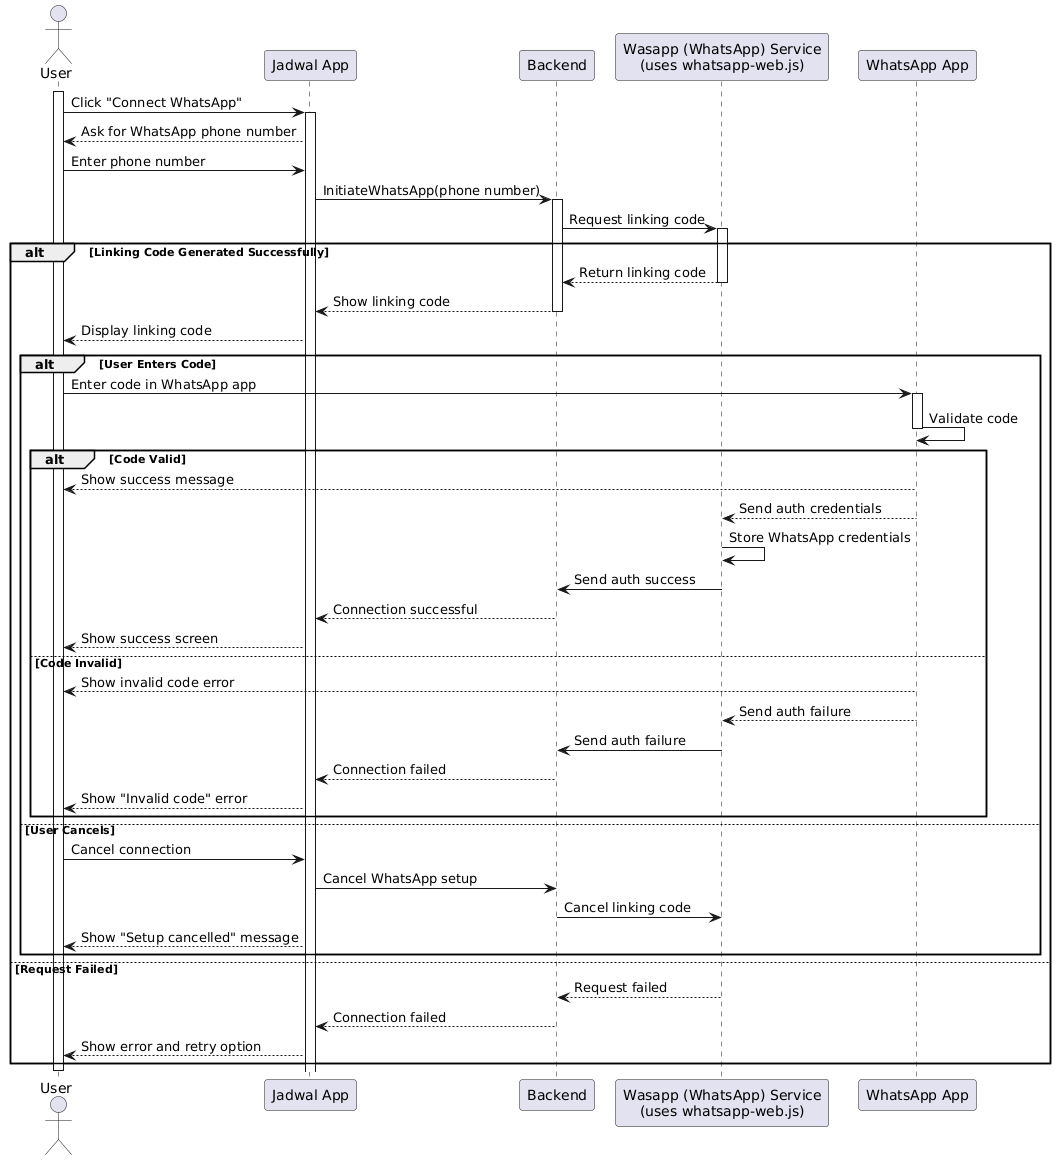
\includegraphics[width=\textwidth]{images/docs/diagrams/sequence-diagrams/all-sequence-diagrams/Connect WhatsApp.png}
  \caption{Connect WhatsApp Sequence Diagram}
  \label{fig:seq/connect-whatsapp}
\end{figure}